\section{Descripción de las Arquitecturas de Combustión}

\subsection{3.1. Combustores Can-Anulares}

Resulta revelador observar cómo los combustores can-anulares han mantenido una posición dominante en la aviación comercial durante más de cuatro décadas. Su diseño híbrido combina la robustez de las cámaras tubulares individuales con la eficiencia estructural de una carcasa anular exterior. 

Cada liner opera en paralelo, alimentado por swirlers y atomizadores dedicados, mientras comparte el flujo de aire secundario y de dilución a través de una envolvente común. Esta disposición facilita enormemente las operaciones de mantenimiento y permite reemplazar liners individuales sin desmontar el motor completo, una ventaja operativa que los ingenieros de línea aprecian en entornos de alta utilización.

No obstante, cabe matizar que la presencia de paredes inter-cámara introduce pérdidas aerodinámicas y cierta heterogeneidad en la distribución circunferencial de temperatura. En muchos casos estudiados, estas discontinuidades geométricas generan zonas de recirculación no deseadas que afectan la uniformidad del patrón factor a la salida.

\subsection{3.2. Combustores Anulares}

Aunque los enfoques tradicionales han aportado fiabilidad demostrada, los combustores anulares completos representan un salto conceptual hacia la integración total del volumen de combustión. En esta arquitectura, la llama ocupa un anillo continuo alrededor del eje del motor, eliminando por completo las divisiones internas. 

Makida y su equipo en el proyecto TechCLEAN de JAXA documentaron exhaustivamente las ventajas de esta configuración en pruebas a escala real, destacando la superior uniformidad térmica y el mejor aprovechamiento del aire disponible para dilución \cite{Makida2008}. 

Moreno et al. profundizaron posteriormente en el diseño específico para motores de la familia CFM56 mediante simulaciones detalladas, mostrando cómo la geometría continua favorece patrones de flujo más predecibles y reduce significativamente la formación de hotspots \cite{Moreno2024}.

\begin{figure}[h]
\centering
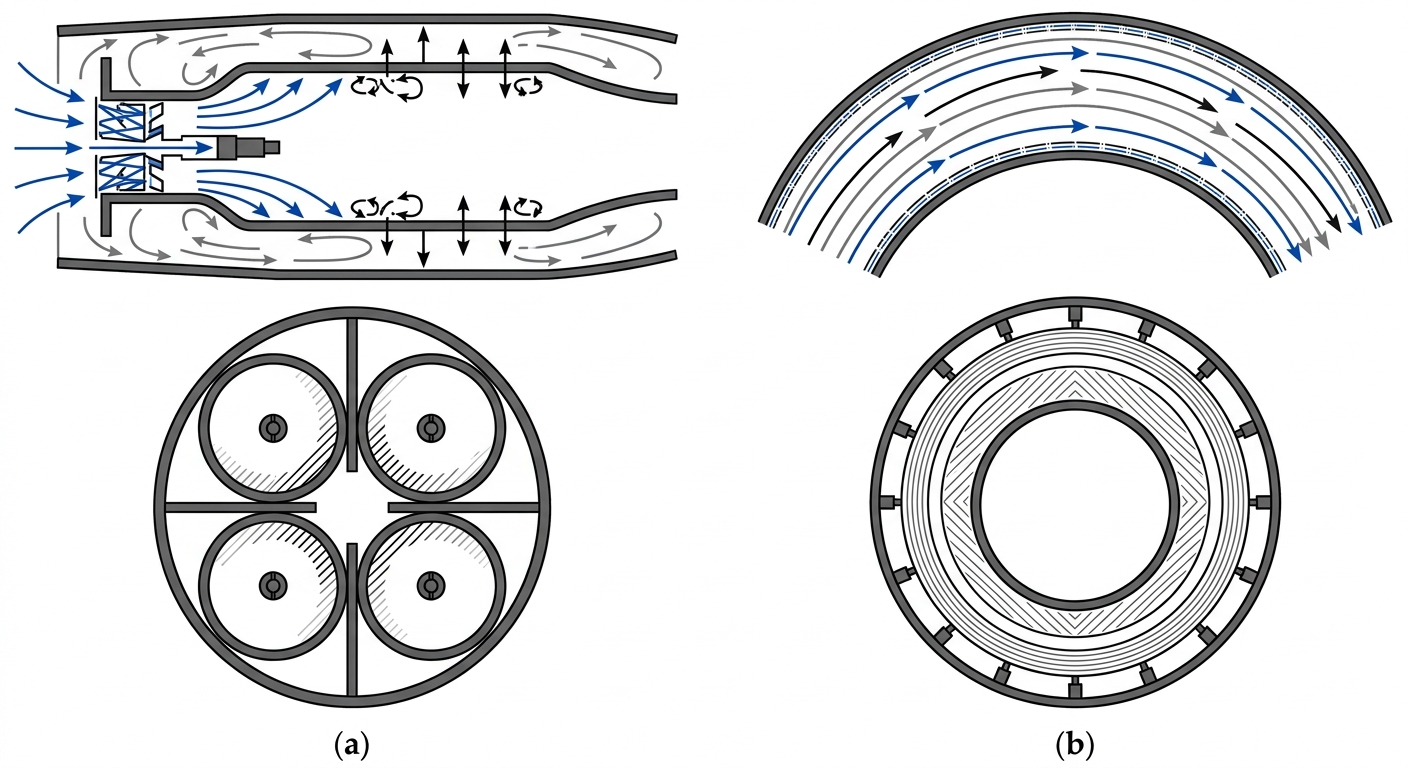
\includegraphics[width=\linewidth]{fig2.png}
\caption{Diagramas esquemáticos comparativos de las arquitecturas: (a) combustor can-anular y (b) combustor anular completo, con indicación de flujos primario, secundario y de dilución.}
\label{fig:diagramas_esquematicos}
\end{figure}

La ecuación principal que gobierna el balance de masa y mezcla en ambos diseños puede expresarse como:

\begin{equation}
\dot{m}_{total} = \dot{m}_{air,prim} + \dot{m}_{fuel} + \dot{m}_{air,sec} + \dot{m}_{dil}
\label{eq:flujo_mezcla}
\end{equation}

donde la distribución porcentual de cada término varía sustancialmente entre arquitecturas, siendo más uniforme en la configuración anular.

\subsection{3.3. Análisis comparativo preliminar de parámetros de diseño}

Uno de los desafíos persistentes que surge al comparar estas arquitecturas radica en la interdependencia entre parámetros geométricos y comportamiento aerotérmico. Los combustores can-anulares suelen presentar relaciones longitud-diámetro más elevadas por liner individual, mientras que los anulares optimizan el espacio anular mediante un menor espesor radial.

Particularmente llamativo es el hecho de que los anulares logren, en promedio, factores de patrón (OTDF) entre 15 y 25\% inferiores a sus contrapartes can-anulares bajo condiciones similares de presión y relación de equivalencia, según los datos reportados por Moreno \cite{Moreno2024}. 

Esta mejora no es gratuita: exige tolerancias de fabricación más estrictas y sistemas de enfriamiento más sofisticados en las paredes internas y externas del anillo. 

Lejos de ser un asunto resuelto, la literatura reciente parece sugerir que la elección óptima depende fuertemente del ciclo termodinámico del motor y del tipo de combustible previsto. Mientras los can-anulares mantienen ventajas claras en costos de desarrollo y certificación incremental, los anulares ofrecen un camino más prometedor hacia las metas de eficiencia y emisiones que la industria debe alcanzar antes de 2035. El resto del artículo profundizará en estas diferencias mediante análisis cuantitativo sistemático.